\renewcommand*{\arraystretch}{1.1}

\subsection*{BI / read / 20}
\label{section:bi-read-20}

\noindent\begin{tabularx}{\queryCardWidth}{|>{\queryPropertyCell}p{\queryPropertyCellWidth}|X|}
	\hline
	query & BI / read / 20 \\ \hline
%
	title & High-level topics
 \\ \hline
%
	pattern & \hfill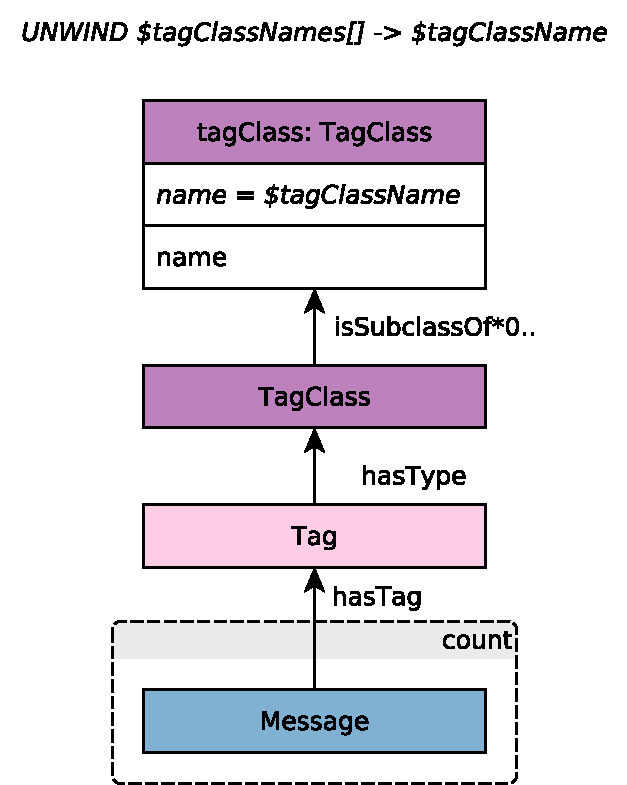
\includegraphics[scale=\patternscale,margin=0cm .2cm]{patterns/bi-read-20}\hfill\vadjust{} \\ \hline
%
	desc. & For all given TagClasses, count number of Messages that have a Tag that
belongs to that TagClass or any of its children (all descendants through
a transitive relation).
 \\ \hline
%
	
		params &
		\innerCardVSpace{\begin{tabularx}{\attributeCardWidth}{|>{\paramNumberCell}c|>{\varNameCell}M|>{\typeCell}m{\typeWidth}|Y|} \hline
		$\mathsf{1}$ & tagClasses
 & String{[}{]}
 &  \\ \hline
		\end{tabularx}}\innerCardVSpace \\ \hline
	
%
	
		result &
		\innerCardVSpace{\begin{tabularx}{\attributeCardWidth}{|>{\resultNumberCell}c|>{\varNameCell}M|>{\typeCell}m{\typeWidth}|>{\resultOriginCell}c|Y|} \hline
		$\mathsf{1}$ & tagClass.name
 & String
 & R &
				The TagClass of the root
 \\ \hline
		$\mathsf{2}$ & postCount
 & 32-bit Integer
 & R &
				 \\ \hline
		\end{tabularx}}\innerCardVSpace \\ \hline
	
%
	
		sort		&
		\innerCardVSpace{\begin{tabular}{|>{\sortNumberCell}c|>{\varNameCell}l|>{\directionCell}c|} \hline
		$\mathsf{1}$ & postCount
 & $\desc
$ \\ \hline
		$\mathsf{2}$ & tagClass.name
 & $\asc
$ \\ \hline
		\end{tabular}}\innerCardVSpace \\ \hline
	%
	limit & 100 \\ \hline
	%
	CPs &
	\multicolumn{1}{>{\raggedright}l|}{
		\chokePoint{1.6}, 
		\chokePoint{2.1}, 
		\chokePoint{6.1}
		} \\ \hline
	%
	%
\end{tabularx}
\queryCardVSpace